\section{The Slice Language and Type System}\label{sec:language}

\begin{figure}[h]
\begin{align*}
e ::= &\; x                               & \text{variable} \\
    | &\; c                               & \text{float constant} \\
    | &\; \text{true} \mid \text{false}   & \text{boolean constant} \\
    | &\; \finconst{k}{n}                 & \text{finite type constant (k of type fin(n))} \\
    | &\; ()                              & \text{unit} \\
    | &\; \letkw \; x = e_1\; \inkw \; e_2  & \text{let binding} \\
    | &\; \text{cdistr}                   & \text{continuous distribution} \\
    | &\; \discrete(p_0, \ldots, p_{n})      & \text{discrete distribution} \\
    | &\; e_1 < e_2                       & \text{less-than (floats)} \\
    | &\; e_1 \leq e_2                    & \text{less-or-equal (integers)} \\
    | &\; e_1 \finlt{n} e_2              & \text{less-than (finite type n)} \\
    | &\; e_1 \finleq{n} e_2             & \text{less-or-equal (finite type n)} \\
    | &\; e_1 \logand e_2                 & \text{logical and} \\
    | &\; e_1 \logor e_2                  & \text{logical or} \\
    | &\; \text{not}\; e                  & \text{logical not} \\
    | &\; \ifkw \; e_1\; \thenkw \; e_2\; \elsekw \; e_3 & \text{conditional} \\
    | &\; (e_1, e_2)                      & \text{pair construction} \\
    | &\; \fstkw \; e                     & \text{first projection} \\
    | &\; \sndkw \; e                     & \text{second projection} \\
    | &\; \funkw \; x \; \rightarrow \; e & \text{function abstraction} \\
    | &\; e_1 \; e_2                      & \text{function application} \\
    | &\; \text{fix}\; f\; x := e         & \text{fixed-point recursion} \\
    | &\; \text{observe}\; e              & \text{observation/conditioning} \\
    | &\; e_1; e_2                        & \text{sequencing} \\
    | &\; \text{nil}                      & \text{empty list} \\
    | &\; e_1 :: e_2                      & \text{list cons} \\
    | &\; \text{match}\; e\; \text{with}\; \text{nil} \rightarrow e_1 \mid h :: t \rightarrow e_2\; \text{end} & \text{list match} \\
    | &\; \text{ref}\; e                  & \text{reference creation} \\
    | &\; !e                              & \text{dereference} \\
    | &\; e_1 := e_2                      & \text{assignment} \\
    \\[1ex] % Add some space before cdistr definition
\text{cdistr} ::= &\; \uniform(e_1, e_2)      & \text{uniform distribution} \\
           | &\; \gaussian(e_1, e_2)   & \text{gaussian distribution} \\
           | &\; \exponential(e)       & \text{exponential distribution} \\
           | &\; \betafn(e_1, e_2)     & \text{beta distribution} \\
           | &\; \ldots                & \text{(and 13+ more distributions)}
\end{align*}
\caption{Syntax of the \Slice{} language.}
\label{fig:grammar}
\end{figure}

The syntax of the \Slice{} language is shown in Figure~\ref{fig:grammar}.
Beyond basic functional constructs, the language includes the following constructs:
\begin{itemize}
\item \textbf{Finite types}: Values of the form $\finconst{k}{n}$ represent finite type constants, where $k$ is a value in the finite type with $n$ elements.
\item \textbf{Discrete distributions}: The $\discrete(p_0, \ldots, p_{n-1})$ construct returns a random value in the finite type with $n$ elements.
\item \textbf{Continuous distributions}: The implementation supports distributions including uniform, Gaussian, exponential, beta, gamma, Laplace, Cauchy, and others.
\item \textbf{Observations}: The $\text{observe}(e)$ construct conditions the program on a boolean expression $e$ being true.
\item \textbf{Other features}: Features such as lists, recursion, and mutable references are supported.
\end{itemize}

When we discretize continuous programs, we convert expressions involving continuous distributions into expressions with discrete distributions over the corresponding finite type, and convert less-than comparisons into less-than-or-equal comparisons on the corresponding discrete values.

\subsection{Type System}\label{sec:type-system}

We introduce a type system that analyzes both the comparison points and concrete values of floating point expressions. We have the following types:
\begin{itemize}
    \item Standard types: $\textbf{int}$, $\textbf{bool}$, $\tau_1 * \tau_2$, $\tau_1 \rightarrow \tau_2$, $\textbf{unit}$, $\textbf{list}(\tau)$, $\textbf{ref}(\tau)$, etc.
    \item $\fin{n}$: finite type with values $\{\finconst{0}{n}, \finconst{1}{n}, \ldots, \finconst{(n-1)}{n}\}$
    \item \float$[B; V]$: floating point type with comparison bounds $B$ and value set $V$ that are elements of the lattice structure described below.
\end{itemize}

\paragraph{Lattice Structure.} 
We use a join-semilattice with the following structure, given a domain $D$:
\begin{itemize}
    \item Elements: $\{\text{Finite}(S) \mid S \text{ is a finite set over } D\} \cup \{\top\}$
    \item Ordering: $\text{Finite}(S_1) \sqsubseteq \text{Finite}(S_2)$ if $S_1 \subseteq S_2$, and $x \sqsubseteq \top$ for any $x$
    \item Join: $\text{Finite}(S_1) \sqcup \text{Finite}(S_2) = \text{Finite}(S_1 \cup S_2)$, and $x \sqcup \top = \top$ for any $x$
    \item Bottom: $\text{Finite}(\emptyset)$
    \item Top: $\top$
\end{itemize}

In $\float$[B; V], $V$ is a lattice element with domain $\R$, and $B$ is a lattice element with domain $<\!\!x$ and $\leq\!\!x$ for all $x \in \R$.
The lattice structure enables type inference to systematically collect and propagate information about both how values are used (bounds) and what values they can take (values).

\begin{figure}[!t]
\centering
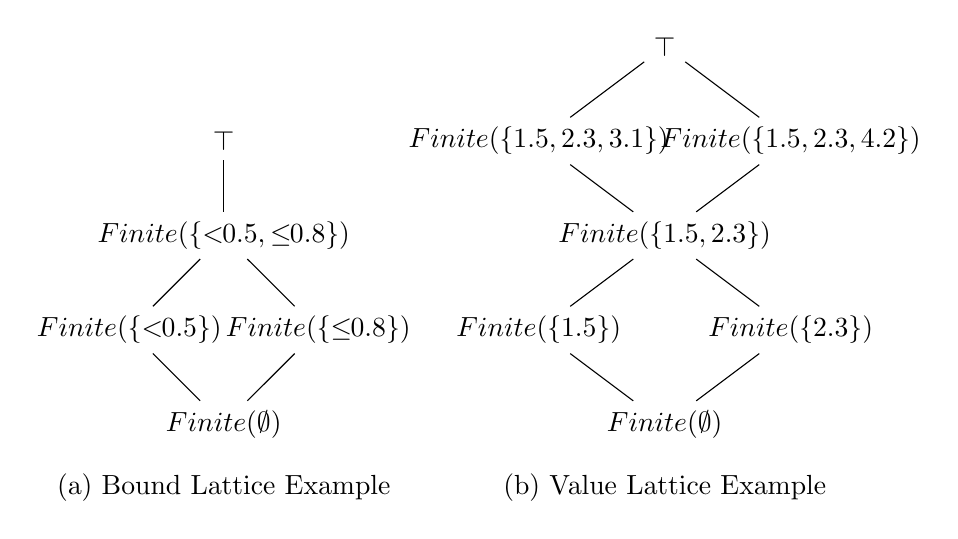
\begin{tikzpicture}[scale=0.8]
  % Individual lattice (left)
  \node (bot1) at (0,0) {$\text{Finite}(\emptyset)$};
  \node (s1) at (-1.5,1.5) {$\text{Finite}(\{<\!\!0.5\})$};
  \node (s2) at (1.5,1.5) {$\text{Finite}(\{\leq\!\!0.8\})$};
  \node (s12) at (0,3) {$\text{Finite}(\{<\!\!0.5, \leq\!\!0.8\})$};
  \node (top1) at (0,4.5) {$\top$};
  
  \draw (bot1) -- (s1);
  \draw (bot1) -- (s2);
  \draw (s1) -- (s12);
  \draw (s2) -- (s12);
  \draw (s12) -- (top1);
  
  \node at (0,-1) {(a) Bound Lattice Example};
  
  % Product lattice (right)
  \node (bot2) at (7,0) {$\text{Finite}(\emptyset)$};
  \node (s3) at (5,1.5) {$\text{Finite}(\{1.5\})$};
  \node (s4) at (9,1.5) {$\text{Finite}(\{2.3\})$};
  \node (s34) at (7,3) {$\text{Finite}(\{1.5, 2.3\})$};
  \node (s5) at (5,4.5) {$\text{Finite}(\{1.5, 2.3, 3.1\})$};
  \node (s6) at (9,4.5) {$\text{Finite}(\{1.5, 2.3, 4.2\})$};
  \node (top2) at (7,6) {$\top$};
  
  \draw (bot2) -- (s3);
  \draw (bot2) -- (s4);
  \draw (s3) -- (s34);
  \draw (s4) -- (s34);
  \draw (s34) -- (s5);
  \draw (s34) -- (s6);
  \draw (s5) -- (top2);
  \draw (s6) -- (top2);
  \node at (7,-1) {(b) Value Lattice Example};
\end{tikzpicture}
\caption{Lattice structure for float types. (a) shows an example bound lattice with comparison bounds. (b) the lattice over real values.}
\label{fig:lattice}
\end{figure}

The typing rules are split into two parts: rules specific to float types and continuous distributions (Figure~\ref{fig:typing-float}), and standard rules for all other language constructs (Figure~\ref{fig:typing-general}).

To understand the float typing rules, it is helpful to understand how discretization works.
A type $\float$[B; V] is discretized as follows:
\begin{itemize}
    \item If $B$ is a finite set of bounds, then the type is discretized to a type $\fin{(n+1)}$ where $n$ is the number of bounds. For instance, if $B = \{<\!\!0.5, \leq\!\!0.8\}$, then the type is discretized to $\fin{3}$, where $\finconst{0}{3}$ represents the range $(-\infty, 0.5)$, $\finconst{1}{3}$ represents the range $[0.5, 0.8]$, and $\finconst{2}{3}$ represents the range $(0.8, \infty)$.
    \item If $B = \top$, then no discretization is performed, and the type remains $\float$.
\end{itemize}

To understand the typing rules, keep in mind that the $B$ set needs to be sufficiently refined (i.e., contain enough comparison points) so that the discretized program has enough information to determine how the original continuous program behaved.

\paragraph{Continuous distributions.} Let us first consider the typing rule for single-argument continuous distributions.
The rule states that the argument $\Gamma \vdash e : \float[B; V]$ with the constraint that $B$ distinguishes $V$. The distinguishes predicate is defined as follows:
\begin{definition}
    \label{def:distinguishes}
    $B$ distinguishes $V$ if every interval in $B$ contains at most one value in $V$, or $B = \top$.
\end{definition}
Intuitively $V$ contains the possible values that the float expression can take on, and $B$ distinguishes $V$ if the continuous quantity can be fully recovered by the discretized program.
For example, if $B = \{<\!\!0.5, \leq\!\!0.8\}$ and $V = \{0.2, 0.7\}$, then $B$ distinguishes $V$. The intervals induced by $B$ are $(-\infty, 0.5)$, $[0.5, 0.8]$, and $(0.8, \infty)$. The first interval contains $0.2$, the second contains $0.7$, and the third contains no values from $V$, so the condition holds. In contrast, if $V = \{0.2, 0.3\}$, $B$ would not distinguish $V$ because both values lie in the first interval $(-\infty, 0.5)$.

Note that if $e$ is a constant, then $V = \{e\}$ and $B = \emptyset$ distinguishes $V$ (because $V$ is a singleton set, so there are no two elements that could lie in the same interval).
If $V = \top$ then $V$ essentially contains all possible real values, so we must also have $B = \top$ in that case.

The rule for two-argument continuous distributions is similar, but the argument $\Gamma \vdash e_1 : \float[B_1; V_1]$ and $\Gamma \vdash e_2 : \float[B_2; V_2]$ with the constraint that $B_1$ and $B_2$ distinguish $V_1$ and $V_2$ respectively.



\paragraph{Comparisons.} 
To understand the typing rules for less-than and less-than-or-equal comparisons, let us first consider a comparison $e < c$ where $c$ is a constant and $e$ is a continuously ranging quantity. Intuitively, if $e : \float[B_1; V_1]$ is discretized, then it must still contain enough information to determine whether $e < c$ is true or false. Therefore, $B_1$ must contain the comparison $<\!\!c$.

Similarly, if $c$ is not a literal constant, but has type $c : \float[B_2; V_2]$, then $c$ can take on values in $V_2$. Therefore, if $V = \{v_1, v_2, \dots, v_n\}$ then $B_1$ must contain the comparisons $<\!\!v_1, <\!\!v_2, \dots, <\!\!v_n$. This motivates the following definition:

\begin{definition}
    \label{def:answers-less}
    $B$ answers $<\!\!V$ if $B$ contains comparisons $<\!\!v$ for every $v \in V$, or $B = \top$.
\end{definition}

In the case that $B = \top$, the quantity is not discretized, so the comparison remains continuous.

Lastly, in order to be able to perform the comparison on the discrete values, we insist that $B_1 = B_2$, ensuring that $e$ and $c$ are discretized to the same representation, and $<$ can be discretized to $\finleq{k}$.

It can also be the case that we have a comparison $c < e$ where the continuously ranging quantity $e : \float[B_2; V_2]$ is on the right hand side. In this case, $B_2$ must answer $c\!\!<$, that is, it must contain a comparison $\leq\!\!c$. To make this explicit, consider $2.3 < e$. We can answer this precisely when $B_2$ contains an intervals $(-\infty, 2.3]$ and $(2.3, +\infty)$: the comparison $2.3 < e$ is true if $e$ is in the second interval, and false if $e$ is in the first interval. Of course, it is also ok if $B_2$ is even more precise, as long as it contains the comparison $\leq\!\!2.3$.

\begin{definition}
    \label{def:answers-less-equal}
    $B$ answers $\leq\!\!V$ if $B$ contains comparisons $\leq\!\!v$ for every $v \in V$, or $B = \top$.
\end{definition}

For less-than-or-equal comparisons, the typing rule is similar, but with the conditions reversed.






\begin{figure}
\begin{mathpar}
    \inferrule[\textsc{Float-Const}]
    {\ c \in V \text{ or } V = \top}
    {\Gamma \vdash c : \float[B; V]}

    \inferrule[\textsc{Continuous-1}]
    {\ \Gamma \vdash e : \float[B_1; V_1] \text{ and } B_1 \textit{ distinguishes } V_1}
    {\Gamma \vdash \exponential(e) : \float[B; \top]}

    \inferrule[\textsc{Continuous-2}]
    {\ \Gamma \vdash e_1 : \float[B_1; V_1] \text{ and } B_1 \textit{ distinguishes } V_1 \and 
       \Gamma \vdash e_2 : \float[B_2; V_2] \text{ and } B_2 \textit{ distinguishes } V_2}
    {\Gamma \vdash \gaussian(e_1, e_2) : \float[B; \top]}

    \inferrule[\textsc{Less}]
    {\Gamma \vdash e_1 : \float[B; V_1] \and \Gamma \vdash e_2 : \float[B; V_2] \and B \textit{ answers} <\!\!V_2 \text{ or } B \textit{ answers} \leq\!\!V_1}
    {\Gamma \vdash e_1 < e_2 : \bool}

    \inferrule[\textsc{Less-Equal}]
    {\Gamma \vdash e_1 : \float[B; V_1] \and \Gamma \vdash e_2 : \float[B; V_2] \and B \textit{ answers} \leq\!\!V_2 \text{ or } B \textit{ answers} <\!\!V_1}
    {\Gamma \vdash e_1 \leq e_2 : \bool}

\end{mathpar}
\caption{Typing rules for float types and continuous distributions. The notions \emph{distinguishes} and \emph{answers} are defined in Definitions~\ref{def:distinguishes} and \ref{def:answers-less} and \ref{def:answers-less-equal}.}
\label{fig:typing-float}
\end{figure}

\begin{figure}
\begin{mathpar}
    \inferrule[\textsc{Var}]
    {\ }
    {\Gamma, x: \tau \vdash x : \tau}

    \inferrule[\textsc{Let}]
    {\Gamma \vdash e_1 : \tau_1 \\
     \Gamma, x: \tau_1 \vdash e_2 : \tau_2}
    {\Gamma \vdash \letkw \; x = e_1 \; \inkw \; e_2 : \tau_2}

    \inferrule[\textsc{If}]
    {\Gamma \vdash e_1 : \bool \\
     \Gamma \vdash e_2 : \tau \\
     \Gamma \vdash e_3 : \tau}
    {\Gamma \vdash \ifkw \; e_1 \; \thenkw \; e_2 \; \elsekw \; e_3 : \tau}

    \inferrule[\textsc{Discrete}]
    {\ }
    {\Gamma \vdash \discrete(p_0, \ldots, p_n) : \fin{n}}

    \inferrule[\textsc{LessEq}]
    {\Gamma \vdash e : \intty}
    {\Gamma \vdash e \leq i : \bool}

    \inferrule[\textsc{Pair}]
    {\Gamma \vdash e_1 : \tau_1 \\
     \Gamma \vdash e_2 : \tau_2}
    {\Gamma \vdash (e_1, e_2) : \tau_1 * \tau_2}

    \inferrule[\textsc{Fst}]
    {\Gamma \vdash e : \tau_1 * \tau_2}
    {\Gamma \vdash \fstkw \; e : \tau_1}

    \inferrule[\textsc{Snd}]
    {\Gamma \vdash e : \tau_1 * \tau_2}
    {\Gamma \vdash \sndkw \; e : \tau_2}

    \inferrule[\textsc{Fun}]
    {\Gamma, x: \tau_1 \vdash e : \tau_2}
    {\Gamma \vdash \funkw \; x \; \rightarrow \; e : \tau_1 \rightarrow \tau_2}

    \inferrule[\textsc{App}]
    {\Gamma \vdash e_1 : \tau_1 \rightarrow \tau_2 \\
     \Gamma \vdash e_2 : \tau_1}
    {\Gamma \vdash e_1 \; e_2 : \tau_2}

    \inferrule[\textsc{True}]
    {\ }
    {\Gamma \vdash \text{true} : \bool}

    \inferrule[\textsc{False}]
    {\ }
    {\Gamma \vdash \text{false} : \bool}

    \inferrule[\textsc{And}]
    {\Gamma \vdash e_1 : \bool \\
     \Gamma \vdash e_2 : \bool}
    {\Gamma \vdash e_1 \logand e_2 : \bool}

    \inferrule[\textsc{Or}]
    {\Gamma \vdash e_1 : \bool \\
     \Gamma \vdash e_2 : \bool}
    {\Gamma \vdash e_1 \logor e_2 : \bool}

    \inferrule[\textsc{Not}]
    {\Gamma \vdash e : \bool}
    {\Gamma \vdash \text{not}\; e : \bool}

    \inferrule[\textsc{Unit}]
    {\ }
    {\Gamma \vdash () : \text{unit}}

    \inferrule[\textsc{FinConst}]
    {0 \leq k < n}
    {\Gamma \vdash \finconst{k}{n} : \fin{n}}

    \inferrule[\textsc{FinLess}]
    {\Gamma \vdash e_1 : \fin{n} \\
     \Gamma \vdash e_2 : \fin{n}}
    {\Gamma \vdash e_1 \finlt{n} e_2 : \bool}

    \inferrule[\textsc{FinLessEq}]
    {\Gamma \vdash e_1 : \fin{n} \\
     \Gamma \vdash e_2 : \fin{n}}
    {\Gamma \vdash e_1 \finleq{n} e_2 : \bool}

    \inferrule[\textsc{Observe}]
    {\Gamma \vdash e : \bool}
    {\Gamma \vdash \text{observe}\; e : \text{unit}}

    \inferrule[\textsc{Seq}]
    {\Gamma \vdash e_1 : \tau_1 \\
     \Gamma \vdash e_2 : \tau_2}
    {\Gamma \vdash e_1; e_2 : \tau_2}

    \inferrule[\textsc{Fix}]
    {\Gamma, f: \tau_1 \rightarrow \tau_2, x: \tau_1 \vdash e : \tau_2}
    {\Gamma \vdash \text{fix}\; f\; x := e : \tau_1 \rightarrow \tau_2}

    \inferrule[\textsc{Nil}]
    {\ }
    {\Gamma \vdash \text{nil} : \text{list}(\tau)}

    \inferrule[\textsc{Cons}]
    {\Gamma \vdash e_1 : \tau \\
     \Gamma \vdash e_2 : \text{list}(\tau)}
    {\Gamma \vdash e_1 :: e_2 : \text{list}(\tau)}

    \inferrule[\textsc{Match}]
    {\Gamma \vdash e : \text{list}(\tau_1) \\
     \Gamma \vdash e_1 : \tau_2 \\
     \Gamma, h: \tau_1, t: \text{list}(\tau_1) \vdash e_2 : \tau_2}
    {\Gamma \vdash \text{match}\; e\; \text{with}\; \text{nil} \rightarrow e_1 \mid h :: t \rightarrow e_2\; \text{end} : \tau_2}

    \inferrule[\textsc{Ref}]
    {\Gamma \vdash e : \tau}
    {\Gamma \vdash \text{ref}\; e : \text{ref}(\tau)}

    \inferrule[\textsc{Deref}]
    {\Gamma \vdash e : \text{ref}(\tau)}
    {\Gamma \vdash !e : \tau}

    \inferrule[\textsc{Assign}]
    {\Gamma \vdash e_1 : \text{ref}(\tau) \\
     \Gamma \vdash e_2 : \tau}
    {\Gamma \vdash e_1 := e_2 : \text{unit}}
\end{mathpar}
\caption{Typing rules for general language constructs}
\label{fig:typing-general}
\end{figure}

